\documentclass{beamer}
\usepackage[utf8]{inputenc}
\usepackage{graphicx}
 \DeclareGraphicsExtensions{.pdf,.png}

\title{Terrorist-sympathizer Networks on Twitter}
\author
{Fred Boehm\inst{1} \and Micah Dillard\inst{2}}
 
\institute % (optional)
{
  \inst{1}%
  Department of Statistics\\
  University of Wisconsin--Madison
  \and
  \inst{2}%
  Department of Political Science\\
  University of Wisconsin--Madison
}



\begin{document}

\frame{\titlepage}

\begin{frame}{Motivation}
 \begin{itemize}
\item Twitter is increasingly becoming an important tool of propaganda, radicalization, and recruitment for terrorist organizations...
    \begin{itemize}
    \item  because they can cheaply disseminate their ideology and actions through \alert{networks of friends and sympathizers}.
    \end{itemize}
\item  This is worrisome because it provides lower risk opportunities for people vulnerable to radicalization to passively and actively volunteer.
\end{itemize}
 
\end{frame}


\begin{frame}{2013 attack of Westgate Mall in Nairobi, Kenya}
           \begin{figure}
            \centering
            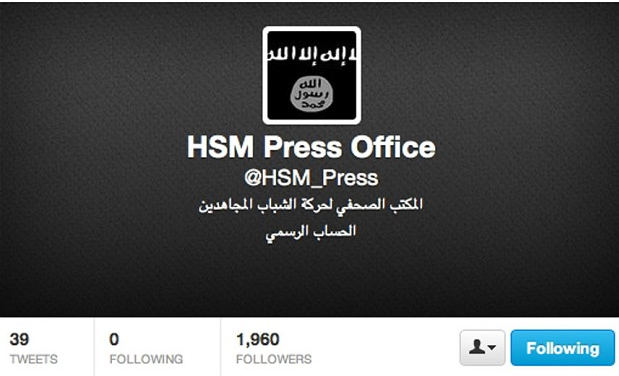
\includegraphics[width=.4\textwidth]{picture3}
            \end{figure}
\begin{itemize}
\item al-Shabaab during  on Westgate Mall in Nairobi, Kenya gave live commentary of its actions on Twitter.
    \begin{itemize}
    \item "The Mujahideen (‘holy warriors’) entered Westgate mall today at around noon and they are still inside the mall, fighting the Kenyan kuffar (‘infidels’) inside their own turf” (Weimann 2014:8)
    \end{itemize} 
\item This was the first time that a group that had mounted a terrorist operation used Twitter to claim responsibility for it (Alexander 2013).
\end{itemize}

\end{frame}

\begin{frame}{Goals}

\begin{itemize}
\item Substantive
    \begin{itemize}
    \item What is the network structure within various organizations' sympathizers (al-Shabaab, ISIS/L, al-Queda, etc.)?
    \item How are individuals connected across groups that they purport to support?
        \begin{itemize}
        \item Twitter allows sympathizers to support and spread information for multiple organizations simultaneously. 
        \end{itemize}
    \end{itemize}
\item Methodological 
    \begin{itemize}
    \item Can we adapt respondent-driven sampling to this setting?
    \item What are useful network parameters that we’d like to estimate?
    \end{itemize}
\end{itemize}

\end{frame}

\begin{frame}{Goals}
\begin{itemize}
\item Substantive
    \begin{itemize}
    \item \alert{What is the network structure within various organizations' sympathizers (al-Shabaab, ISIS/L, al-Queda, etc.)?}
    \item How are individuals connected across groups that they purport to support?
    \end{itemize}
\item Methodological 
    \begin{itemize}
    \item Can we adapt respondent-driven sampling to this setting?
    \item \alert{What are useful network parameters that we’d like to estimate?}
    \end{itemize}
\end{itemize}
\end{frame}

\begin{frame}{Methods}
\begin{itemize}

\item We accessed Twitter data (lists of friends and friends) with the SMAPPR package in R.
    \begin{itemize}
    \item Twitter permits us to see the entirety of a given user’s friends \& friends
    \end{itemize}
\item Our measure of connectivity is the Jaccard index
    \begin{itemize}
    \item Jaccard index is defined, for a pair of sets, A and B, as the ratio of the cardinality of the intersection to the cardinality of the union
    \end{itemize}
\end{itemize}

\end{frame}

\begin{frame}{Methods}
\begin{itemize}

  \item Collect the list of friends of a seed account
  \item \pause Randomly sample 2 friends, A and B
  \item \pause Collect the list of friends of A and B
  \item \pause Calculate the Jaccard index for friends of A and B  
  \item \pause  Repeat for another random sample of two friends or friends
\end{itemize}

\end{frame}

\begin{frame}{Results}
\begin{columns}
        \begin{column}{0.5\textwidth}
            \begin{itemize}
\item @WaleedGaj2002 (confirmed al-Queda)
    \begin{itemize}
    \item Two of 688  friends chosen randomly
    \item Jaccard index for friends of A and friends of B calculated (Repeat 1500 times)
        \begin{itemize}
        \item Number with nonzero Jaccard index: 658
        \item Number with Jaccard index greater than 0.1: 13
        \end{itemize}
    \end{itemize}
\end{itemize}
        \end{column}
        \begin{column}{0.5\textwidth}
            \begin{figure}
            \centering
            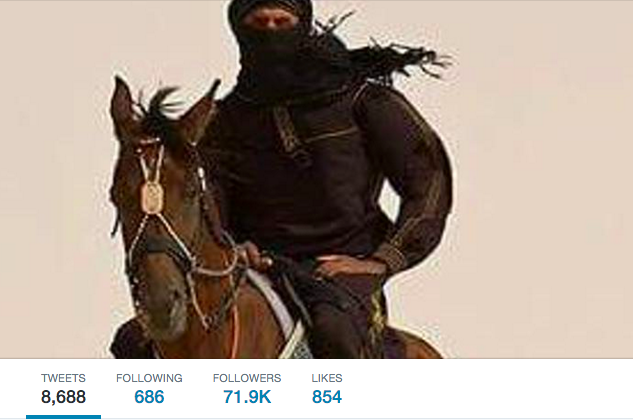
\includegraphics[width=1\textwidth]{picture}
            \caption{@WaleedGaj2002's cover photo}
            \end{figure}
        \end{column}
    \end{columns}
\end{frame}

\begin{frame}{Results}
\begin{columns}
        \begin{column}{0.5\textwidth}
           \begin{figure}
            \centering
            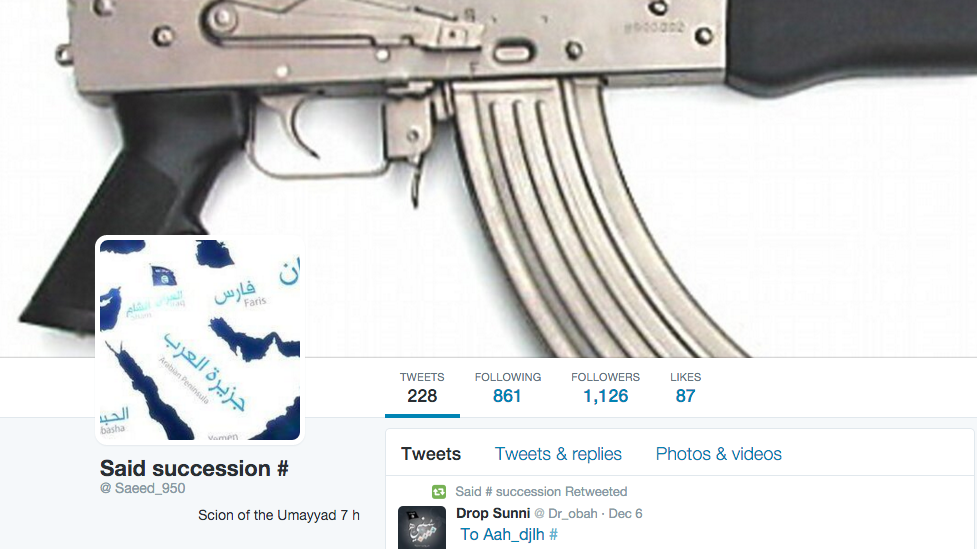
\includegraphics[width=1\textwidth]{picture2}
            \caption{@saeed\_950's cover photo}
            \end{figure}
        \end{column}
        \begin{column}{0.5\textwidth}
            \begin{itemize}
\item @WaleedGaj2002 and @saeed\_950 (suspected ISIS-affiliate with 1125 friends) 
    \begin{itemize}
    \item Intersection of 8 friends
    \item Jaccard index of .0053
    \end{itemize}
\item Some of these 8 individuals are journalists of some sort. Highlighting the problem of identification. 
\end{itemize}

        \end{column}
    \end{columns}
\end{frame}



\end{frame}

\begin{frame}{Results}

\begin{itemize}
\item @WaleedGaj2002 and @saeed\_950
    \begin{itemize}
    \item @WaleedGaj2002's friends and @saeed\_950's followers
        \begin{itemize}
        \item Jaccard index of 0
        \end{itemize}
    \item @WaleedGaj2002's followers and @saeed\_950's friends
        \begin{itemize}
        \item Intersection = 39, union = 72,707, and Jaccard index = .0005364
        \end{itemize}
    \end{itemize}
\item We speculate that @WaleedGaj2002 is more relevant than @saeed\_950 because @saeed\_950's friends follows @WaleedGaj2002 but the opposite is not true.
\end{itemize}

\end{frame}

\begin{frame}{Limitations}
\begin{itemize}
\item Twitter actively disables accounts of terrorists and criteria for disabling are not clear
\item API can be accessed, on average, once per minute
\item The problem of identification. 
\end{itemize}
\begin{figure}
\centering
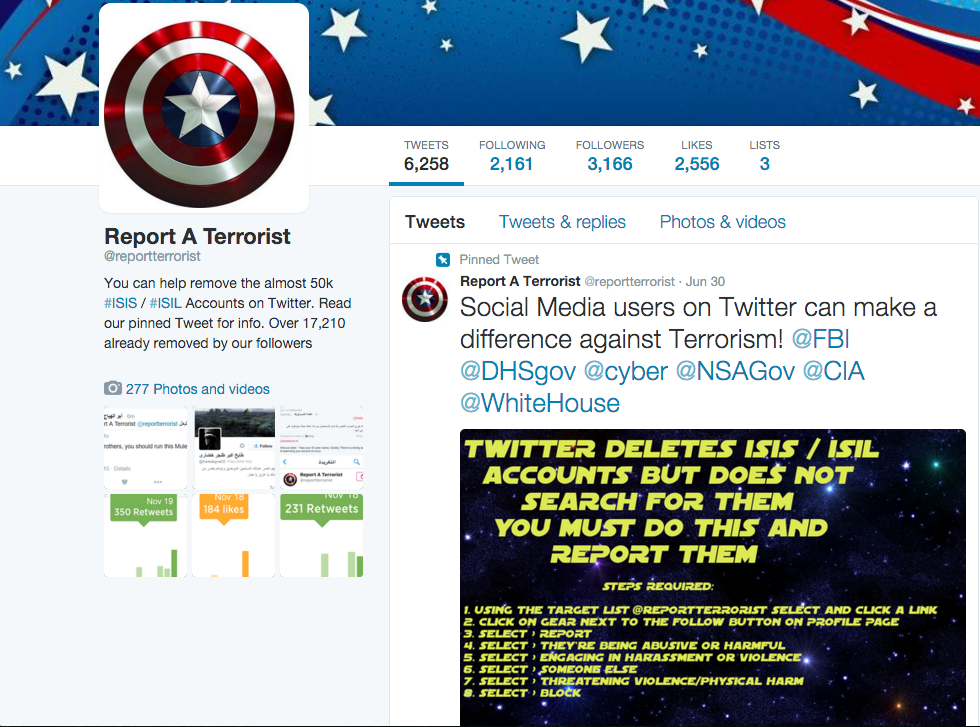
\includegraphics[width=1\textwidth]{picture1}
\end{figure}

\end{frame}

\end{document}
\\
